{}\documentclass[letterpaper,
compress,
xcolor=x11names,
%draft,
]{beamer}
% Package imports
\usepackage{mathtools} % imports `amsmath'
\DeclareMathOperator{\sech}{sech}
\usepackage{amssymb}
\usepackage{fixltx2e}
\usepackage{lmodern}
\usepackage{movie15}
%\usepackage{media9}
\usepackage{microtype}
\usepackage{animate}
\usepackage{subcaption}
\captionsetup{compatibility=false}

% I just did this
\usepackage[english]{babel}
\usepackage[utf8]{inputenc}
\usepackage{amsmath}
\usepackage{graphicx}
\usepackage[colorinlistoftodos]{todonotes}
\usepackage{tikz}
\usetikzlibrary{tikzmark}
\usepackage{array}
\usepackage{layout}
\usepackage{multicol}
\usepackage{multirow}
\usepackage{booktabs}
%I just did this

% `beamer' configuration
\usefonttheme{professionalfonts}
\useoutertheme[subsection=false,]{miniframes}
\setbeamercolor*{alerted text}{fg=red}
\setbeamercolor*{example text}{fg=black}
\definecolor{CSU_green}{RGB}{30, 70, 43}
\definecolor{CSU_gold}{RGB}{200, 195, 114}
\setbeamercolor*{lower separation line head}{bg=CSU_gold}
\setbeamercolor*{section in head/foot}{fg=white,bg=CSU_green}
\setbeamercolor*{subsection in head/foot}{bg=white}
\setbeamercolor*{upper separation line head}{bg=CSU_gold}
\setbeamercolor*{page number in head/foot}{fg=CSU_green}
\setbeamercolor*{normal text}{fg=black,bg=white}
\setbeamercolor*{palette tertiary}{fg=black,bg=black!10}
\setbeamercolor*{palette quaternary}{fg=black,bg=black!10}
\setbeamercolor*{structure}{fg=black}
\setbeamerfont{frametitle}{shape=\scshape}
\setbeamerfont{institute}{shape=\scshape}
\setbeamerfont{section in head/foot}{shape=\scshape}
\setbeamerfont{subsection in head/foot}{shape=\scshape}
\setbeamertemplate{bibliography item}{}
\setbeamertemplate{itemize items}[ball]
\setbeamertemplate{navigation symbols}{}
\setbeamertemplate{footline}[frame number]
\usetikzlibrary{calc,arrows}
\graphicspath{{graphics/}{graphics/movies/}{graphics/images/}}
\usepackage{remreset}                  % hack to display beamer navigation
\makeatletter                          % circles even if not declaring
\@removefromreset{subsection}{section} % subsections
\makeatother                           % see: http://tex.stackexchange.com/a/2078
\setcounter{subsection}{1}             % see: https://bitbucket.org/rivanvx/beamer/issue/218

% `biblatex' configuration
\usepackage[backend=biber,
style=authortitle-comp,
]{biblatex}
\addbibresource{presentation.bib}

% `enumitem' configuration
\usepackage{enumitem}
\setlist[itemize,1]{label=\usebeamertemplate{itemize item}}
\setlist[itemize,2]{label=\usebeamertemplate{itemize subitem}}
\setlist[itemize,3]{label=\usebeamertemplate{itemize subsubitem}}
\DeclareMathOperator{\sinc}{sinc}


% `graphicx' configuration
\usepackage{graphicx}
\begin{document}
	\title{Numerical Integration}
	%\subtitle{MATH-151:  Mathematical Algorithms in Matlab}
	\author{MATH-151:  Mathematical Algorithms in Matlab}
	\date[202X]{September 25, 2023}
	\titlegraphic{
\includegraphics[height = 3cm]{CSU_Ram_Logo.jpg}}



%%%%%%%%%%%%%%%%%%%%%%%%%%%%%%%%%%%%%%%%%%%%%%%%%%%%%%

\begin{frame}
\titlepage
\end{frame}
%%%%%%%%%%%%%%%%%%%%%%%%%%%%%%%%%%%%%%%%%%%%%%%%%%%%%%%%%
\section{Quadrature Methods}

\begin{frame}{Integration in Practice}
	\footnotesize
	\begin{itemize}
		\item \underline{Reminder}: The definite integral of a function $f(x)$ between points $a$ and $b$ outputs the area beneath that curve between $x=a$ and $x=b$ and is represented 
		\begin{equation*}
			\int_{a}^{b}f(x)dx
		\end{equation*}
		\item Integrals effectively ``accumulate" the effect of $f$, for a few examples
		\begin{itemize}
			\item Integrating velocity over some time tells us how far an object traveled
			\item The area under a probability distribution gives us a probability
			\item Computing oddly shaped areas and volumes
			\item Often used for solutions of differential equations
		\end{itemize}
		\item There are many different rules for performing these integrals, and many of them are very complicated for a computer to perform, so we find approximations!
	\end{itemize}
	\begin{center}
		\textbf{Ex:} $\displaystyle \int_{0}^{1} e^{-x^2} dx$ \hspace{0.5cm}
		\raisebox{-1cm}{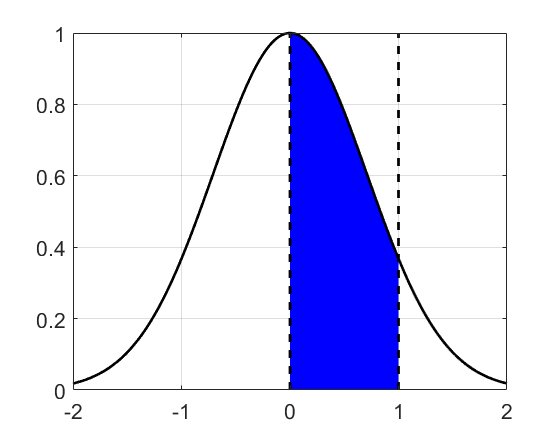
\includegraphics[height = 2.25cm]{integration_ex.png}}
	\end{center}
\end{frame}

%%%%%%%%%%%%%%%%%%%%%%%%%%%%%%%%%%%%%%%%%%%%%%%%%%%%%%%%%%

\begin{frame}{Rectangular Approximations}
	\footnotesize
	\begin{itemize}
		\item A very basic way to quickly approximate an  integral is to assume that the function is constant, $f(x) \approx c$
		\item This is  pretty good because our area will become a rectangle, and we know how to calculate the area of a rectangle! $A = wh$
		\item We have many choices for our $c$, lets look at some popular options
		\begin{itemize}
			\item \textbf{Left-hand rule}, $f(x)\approx f(a)\Rightarrow \displaystyle \int_{a}^{b}f(x)dx\approx (b-a)f(a)$
			\item \textbf{Right-hand rule}, $f(x)\approx f(b)\Rightarrow  \displaystyle \int_{a}^{b}f(x)dx\approx (b-a)f(b)$
			\item \textbf{Midpoint rule}, $f(x)\approx f(\frac{a+b}{2})\Rightarrow  \displaystyle \int_{a}^{b}f(x)dx\approx (b-a)f(\frac{a+b}{2})$
		\end{itemize}
	\end{itemize}
	\begin{center}
		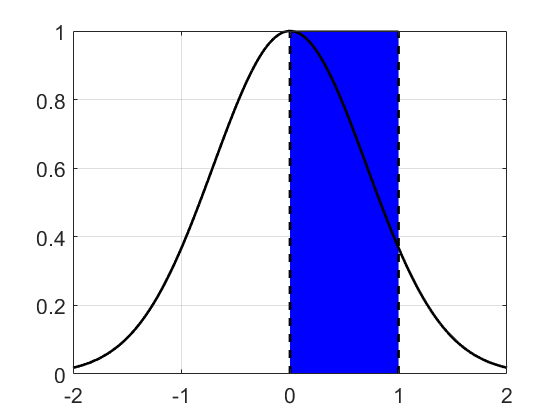
\includegraphics[height = 2.25cm]{left_approx.png} \hspace{0.5cm}
		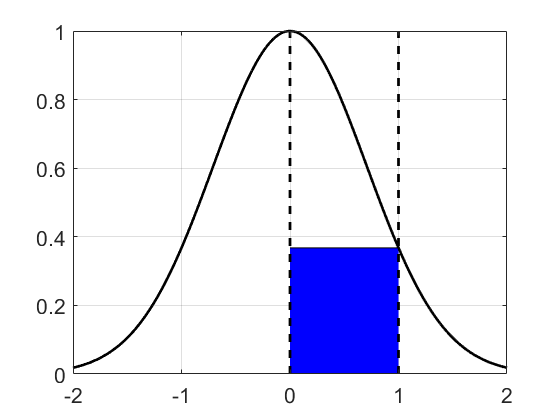
\includegraphics[height = 2.25cm]{right_approx.png} \hspace{0.5cm}
		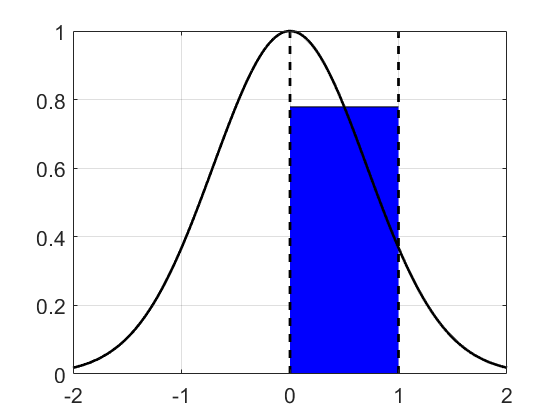
\includegraphics[height = 2.25cm]{center_approx.png} 
	\end{center}
\end{frame}

%%%%%%%%%%%%%%%%%%%%%%%%%%%%%%%%%%%%%%%%%%%%%%%%%%%%%%%%%

\begin{frame}{Trapezoidal Rule}
	\footnotesize
	\begin{itemize}
		\item If we want to allow out function to actually change with varying $x$ values, the next easiest thing we can do is assume the function is a line between $(a,f(a))$ and $(b,f(b))$
		\item We could write this out as a function, but we can think of this as forming a trapezoid with our area. We know how to calculate the area of a trapezoid! $A  = w\frac{h_1+h_2}{2}$ 
		\item This doesn't have any choices so we write it as follows\\
		\textbf{Trapezoidal Rule: } $\int_{a}^{b}f(x)dx\approx (b-a)\frac{f(a)+f(b)}{2}$
	\end{itemize}
	\begin{center}
		\textbf{Ex:} $\displaystyle \int_{0}^{1} e^{-x^2} dx\approx(1-0)\frac{e^{-(0^2)}+e^{-(1^2)}}{2}$ \hspace{0.5cm}
		\raisebox{-1cm}{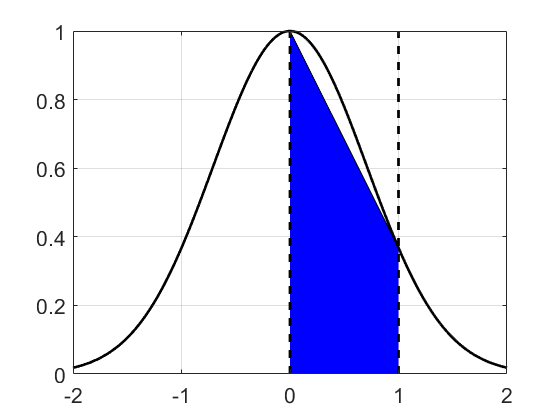
\includegraphics[height = 2.25cm]{trapz_approx.png}}
	\end{center}
\end{frame}

%%%%%%%%%%%%%%%%%%%%%%%%%%%%%%%%%%%%%%%%%%%%%%%%%%%%%%%%%

\begin{frame}{Simpson's Rule}
	\footnotesize
	\begin{itemize}
		\item Now that we have seen interpolation, we can go another step further and find a parabola that goes through our edges and our midpoint $m=\frac{a+b}{2}$. We then find a surprisingly nice formula comes out of that!
		\tiny{
		\begin{align*}
			\displaystyle f(x) &\approx f(a) + \frac{f(m)-f(a)}{\frac{b-a}{2}}(x-a) + \frac{f(b)-2f(m)+f(a)}{\frac{(b-a)^2}{2}}(x-a)(x-m) \\
			\int_{a}^{b}f(x)dx &\approx \int_{a}^{b}\Big(f(a) + \frac{f(m)-f(a)}{\frac{b-a}{2}}(x-a) + \frac{f(b)-2f(m)+f(a)}{\frac{(b-a)^2}{2}}(x-a)(x-m)\Big)dx \\ 
			&= \frac{b-a}{6}(f(a) + 4f(m) + f(b))
		\end{align*}}
		\footnotesize
		\item This gives us \textbf{Simpson's Rule:} $\int_{a}^{b}f(x)dx\approx \frac{b-a}{6}(f(a) + 4f(m) + f(b))$
	\end{itemize}
	\begin{center}
		\textbf{Ex:} $\displaystyle \int_{0}^{1} e^{-x^2} dx\approx\frac{(1-0)}{6}\Big(e^{-(0^2)}+4e^{-(\frac{1}{2}^2)}+e^{-(1^2)}\Big)$ 
		\raisebox{-1cm}{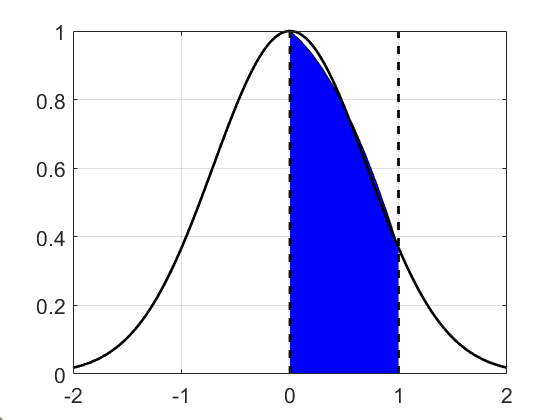
\includegraphics[height = 2.25cm]{simps_approx.png}}
	\end{center}
\end{frame}

%%%%%%%%%%%%%%%%%%%%%%%%%%%%%%%%%%%%%%%%%%%%%%%%%%%%%%%%%
\section{Antiderivatives}

\begin{frame}{Riemann Sums}
	\footnotesize
	\begin{itemize}
		\item If we can get data for many points, we can also make our approximation more accurate by cutting our range into tinier slices!
		\item This is normally referred to as a \textbf{Riemann Sum}
		\item We can use each of the methods above to calculate the areas of each our our slices.
		\begin{itemize}
			\item As we saw from Simpson's rule, we get much better estimates at the cost of needing to know more points.
		\end{itemize}
		\item Here are our Riemann sums using 10 equal sized ``slices"
	\end{itemize}
	\begin{center}
		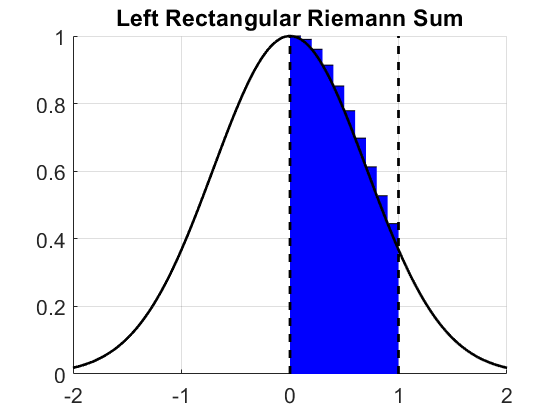
\includegraphics[height = 2.25cm]{left_riemann.png} \hspace{0.5cm}
		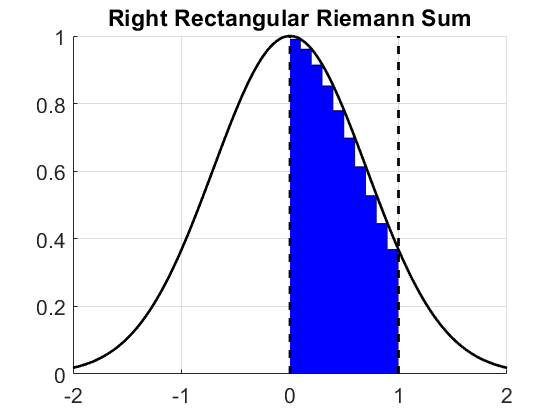
\includegraphics[height = 2.25cm]{right_riemann.png} \hspace{0.5cm}
		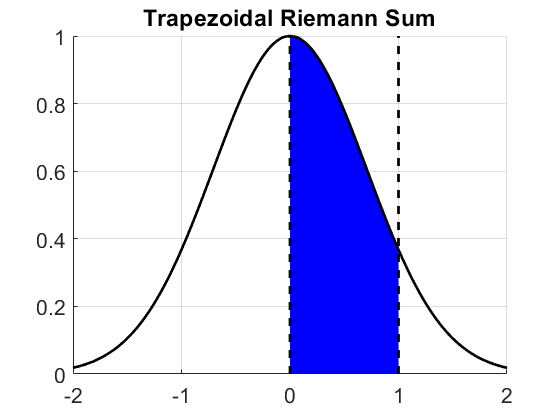
\includegraphics[height = 2.25cm]{trapz_riemann.png}	
	\end{center}
\end{frame}

%%%%%%%%%%%%%%%%%%%%%%%%%%%%%%%%%%%%%%%%%%%%%%%%%%%%%%%%%

\begin{frame}{Estimating the Antiderivative}
	\footnotesize
	\begin{itemize}
		\item Since when we are performing a Riemann sum we are just making approximation of the integral of smaller sections and then adding them together, we can get a sequence of sums.
		\item For example, if we consider our Riemann sum earlier $\int_{0}^{1}e^{-x^2}dx \approx \sum_{n=1}^{10}\frac{1}{10}e^{-\frac{n-1}{10}^2}$ \\
		If we only take the first half half of that sum, we get the integral along half of that range! \\
		$ \sum_{n=1}^{5}\frac{1}{10}e^{-\frac{-1}{10}^2} \approx \int_{0}^{\frac{1}{2}}e^{-x^2}dx$
		\item This sequence can allow us to see an estimate of the antiderivative (plus or minus some constant $C$)
	\end{itemize}
	\begin{center}
		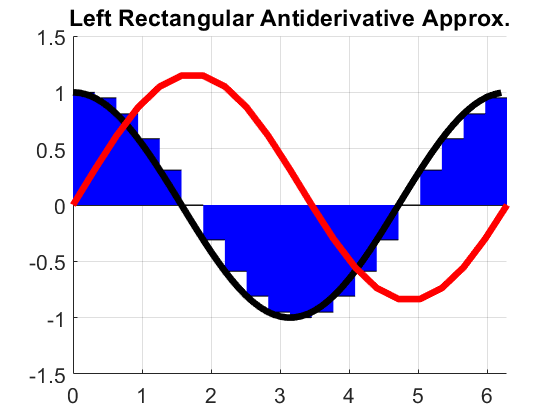
\includegraphics[height = 2.25cm]{left_antideriv_approx.png} \hspace{0.5cm}
		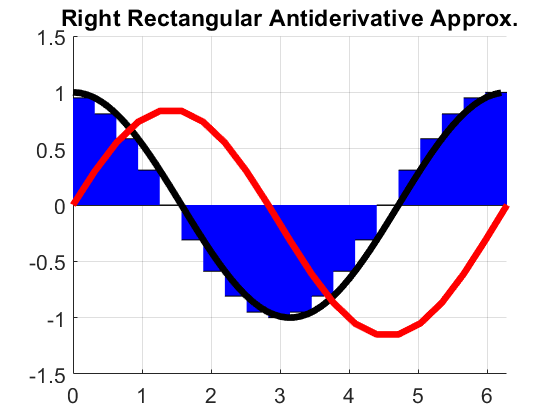
\includegraphics[height = 2.25cm]{right_antideriv_approx.png} \hspace{0.5cm}
		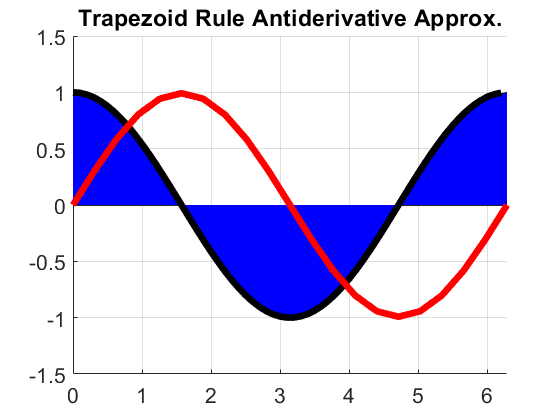
\includegraphics[height = 2.25cm]{trapz_antideriv_approx.png}
	\end{center}
\end{frame}

%%%%%%%%%%%%%%%%%%%%%%%%%%%%%%%%%%%%%%%%%%%%%%%%%%%%%%%%%
\end{document}